%% Based on a TeXnicCenter-Template by Gyorgy SZEIDL.
%%%%%%%%%%%%%%%%%%%%%%%%%%%%%%%%%%%%%%%%%%%%%%%%%%%%%%%%%%%%%

%----------------------------------------------------------
%
\documentclass[titlepage,leqno]{beamer}%
\usetheme{Antibes}%
\usecolortheme{rose}%
\setbeamerfont{footnote}{size=\tiny}
\setbeamercolor{footnotet}{bg=white}
%
%----------------------------------------------------------
% This is a sample document for the LaTeX Slides Class
% Class options
%       --  Body text point size (normalsize) is 27 (default)
%           and can not be adjusted to any other value.
%       --  Paper size:  letterpaper (8.5x11 inch, default)
%                        a4paper, a5paper, b5paper,
%                        legalpaper, executivepaper
%       --  Orientation (portrait is the default):
%                        landscape
%       --  Quality:     final(default), draft
%       --  Title page:  titlepage, notitlepage
%       --  Columns:     onecolumn (default), [twocolumn is not avalible]
%       --  Equation numbering (equation numbers on the right is the default)
%                        leqno (equation numbers on the left)
%       --  Displayed equations (centered is the default)
%                    fleqn (flush left)
%
%  \documentclass[a4paper,fleqn]{slides}
%
%  The slides are separated from each other by the slide
%  environment, see below:
%
%%%
% Some helpful information:
%
% You can typeset \emph{Emphasized text}.
%
% You can also typeset  \textbf{Bold}, \textit{Italics},
% \textsl{Slanted} and \texttt{Typewriter} text. Roman fonts are not
% available.
%
% Point size can be changed by making use of the {\tiny tiny},
% {\scriptsize scriptsize}, {\footnotesize footnotesize}, {\small
% small}, {\normalsize normalsize}, {\large large}, {\Large Large},
% {\LARGE LARGE}, {\huge huge} and {\Huge Huge} commands.
%
% The numbered equation
% \begin{equation}
% u_{tt}-\Delta u+u^{5}+u\left|  u\right|  ^{p-2}=0\text{ in }\mathbf{R}%
% ^{3}\times\left[  0,\infty\right[  .\label{eqn1}%
% \end{equation}
% is automatically numbered as equation \ref{eqn1}.
%%%

\usepackage{amsmath}%
\usepackage{nopageno}%
\usepackage{framed}%
\usepackage{animate}%
\usepackage{amsfonts}%
\usepackage{amssymb}%
\usepackage{graphicx}%
\usepackage{adjustbox}%
\usepackage[utf8]{inputenc} % allow utf-8 input
%\usepackage[T1]{fontenc}    % use 8-bit T1 fonts
\usepackage{hyperref}       % hyperlinks
\usepackage{url}            % simple URL typesetting
\usepackage{booktabs}       % professional-quality tables
\usepackage{nicefrac}       % compact symbols for 1/2, etc.
\usepackage{microtype}      % microtypography
\usepackage{verbatim}

%%  \usepackage{bibentry}
%%  \usepackage{natbib}
%------------------------------------------------------------------
\hfuzz5pt % Don't bother to report overfull boxes < 5pt
\pagestyle{plain}
%%% --------------------------------------------------------------
\begin{document}
\title{MINST Kaggle Digit Recognizer: Contrasting the Random Forest and MLP Neural Network}
\author{%
   Andrew Osborne \hspace{2.75cm} Josh Price\\
   \texttt{amo004@uark.edu} \hspace{1.75cm} \texttt{jdp024@uark.edu} \\
   \vspace{4mm}
   April Walker \\
   \texttt{adw027@uark.edu}
}
\institute{%
   University of Arkansas, \\
   Fayetteville, AR, 72701, USA
	}

\date{4/23/2019}
\maketitle
%-----------------------------------------------------------------
\begin{frame}{Presentation Outline}
	\begin{itemize}
		\item The MINST Dataset
		\item GridSearchCV
		\item Random Forest
		\begin{itemize}
			\item Implementation
			\item Results
		\end{itemize}
		\item Multi-Layer Perception Classifier
		\begin{itemize}
			\item Contrasting Gradient Descent Algorithms
			\item Implementation
			\item Results
		\end{itemize}
		\item{Conclusions}
	\end{itemize}
\end{frame}
% ----------------------------------------------------------------
\begin{frame}{The MINST Dataset}
%The MNIST digit database is a classic starting point for individuals wanting to learn the basics of computer vision and get hands on experience with machine learning algorithms. The dataset is composed of 70,000 28x28 pixel grey-scale images of handwritten numbers between zero and nine [6]. The pre-flattened Kaggle dataset provides you with 42,000 training examples and 28,000 testing examples. Each 28x28 pixel image is represented by a 784 length vector with each element containing some integer between 0 and 255 representing the lightness or darkness of that pixel. Additionally, the training dataset provides the correct labels for each image. These images can be reshaped and rendered from the provided dataset as shown in Figure 1.
\begin{figure}[h]
  \centering
    \begin{minipage}[t]{0.3\textwidth}
        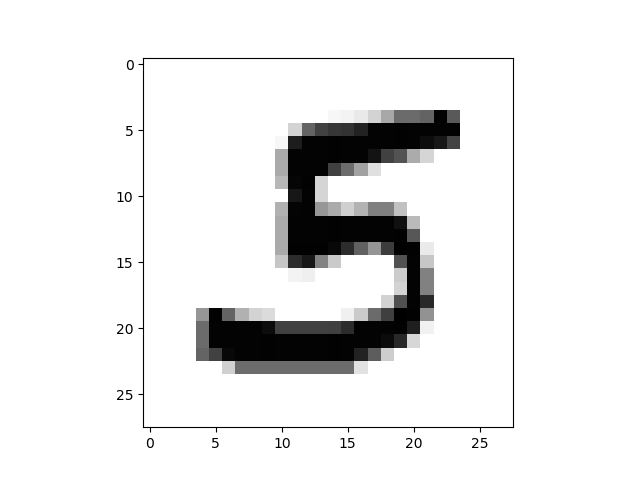
\includegraphics[width=\textwidth]{img786render.png}
    \end{minipage}
    \begin{minipage}[t]{0.3\textwidth}
        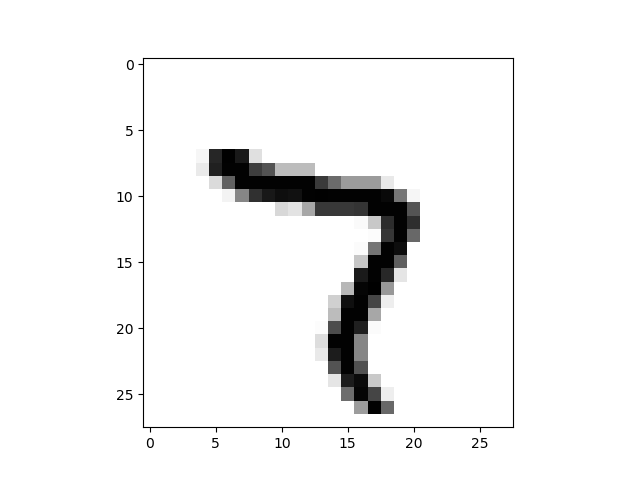
\includegraphics[width=\textwidth]{img98render.png}
    \end{minipage}
    \begin{minipage}[t]{0.3\textwidth}
        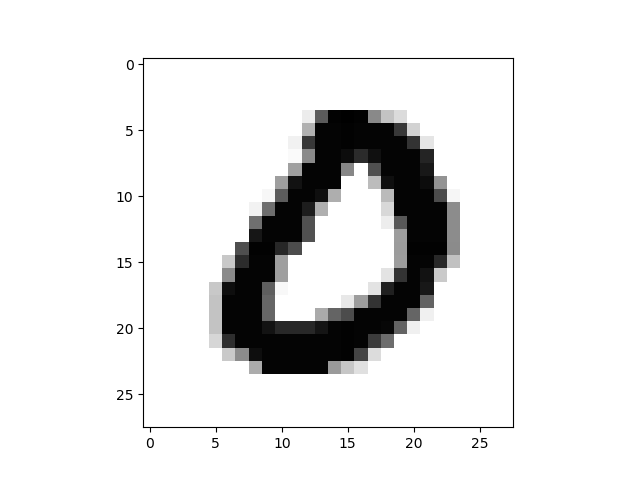
\includegraphics[width=\textwidth]{img6render.png}
    \end{minipage}
  \caption{Image Renderings from the MNIST Dataset}
\end{figure}
\end{frame}
%-----------------------------------------------------------------
\begin{frame}{The MINST Dataset}
\begin{itemize}
	\item 70,000 $28\times 28$ pixel grey-scale images of handwritten numbers, 0 through 9
	\vspace{3.5mm}
	\item Each image is represented by a vector of length 784, with each element taking a value between 0 and 255 to represent lightness/darkness of the pixel
	\vspace{3.5mm}
	\item Pre-flattened Kaggle dataset
	\begin{itemize}
		\item 42,000 training examples
		\item 28,000 testing examples
	\end{itemize}
\end{itemize}
%The MNIST digit database is a classic starting point for individuals wanting to learn the basics of computer vision and get hands on experience with machine learning algorithms. The dataset is composed of 70,000 28x28 pixel grey-scale images of handwritten numbers between zero and nine [6]. The pre-flattened Kaggle dataset provides you with 42,000 training examples and 28,000 testing examples. Each 28x28 pixel image is represented by a 784 length vector with each element containing some integer between 0 and 255 representing the lightness or darkness of that pixel. Additionally, the training dataset provides the correct labels for each image. These images can be reshaped and rendered from the provided dataset as shown in Figure 1.
\end{frame}
%-----------------------------------------------------------------
\begin{frame}[fragile]{GridSearchCV}
\begingroup
\small
For both machine learning algorithms, training and cross-validation was done using \verb+sklearn+'s \verb+model_selection.GridSearchCV+

\vspace{3.75mm}

\verb+GridSearchCV+ partitions the data into $k$ sections then trains the data on $k-1$ of the sections, leaving the last partition as a pseudo-test dataset

\vspace{3.75mm}

The mean cross-validation score (CVS) is the averaged prediction rate over all $k$ segments of the training data, and the hyper-parameter combination with the best mean CVS is chosen

\vspace{3.7mm}

\endgroup
\end{frame}
%-----------------------------------------------------------------
\begin{frame}[fragile]{Random Forest}

Our random forest is a ``highly random'' random forest which splits data with no discretion to promote model volatility

\vspace{3.75mm}

\verb+Sklearn+'s \verb+RandomForestClassifier+ combines the probabilistic prediction of each tree, as this has been shown to preform better than the traditional majority vote approach

\vspace{3.7mm}

These models are generally very fast to train, but depending on the complexity, can suffer from slow classification time

\vspace{3.7mm}

High-dimensional data often poses a problem for Random Forests.

\end{frame}
%-----------------------------------------------------------------
\begin{frame}[fragile]{Random Forest}
\small
\textbf{Implementation}

\medskip

In order to optimize our model's predictive power, we contrasted the results from the following hyper-parameters:
\begin{itemize}
    \item \verb+n_estimators+ (number of trees)
    \item \verb+min_samples_split+ (minimum leaves to split node) % required to split a node
\end{itemize}
\vspace{3.75mm}

Once the code was prepared, training took approximately 45 seconds per model.

\end{frame}
%-----------------------------------------------------------------
\begin{frame}[fragile]{Random Forest}
\small
\textbf{Implementation}

\medskip

In order to optimize our model's predictive power, we contrasted the results from the following hyper-parameters:
\begin{itemize}
    \item \verb+n_estimators+ \{10, 20, 100, 300\}
    \item \verb+min_samples_split+ \{2,4,8,16\}
\end{itemize}
\vspace{3.75mm}

Once the code was prepared, training took approximately 45 seconds per model.

\end{frame}
%-----------------------------------------------------------------
\begin{frame}{Random Forest}

\begin{figure}[h]
    \centering
    \begin{minipage}[t]{0.45\textwidth}
        \centering
        \textbf{(A)}
        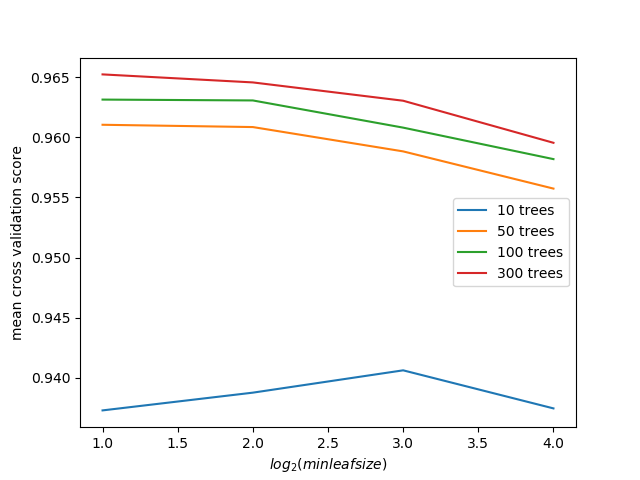
\includegraphics[width=\textwidth]{CVscoreVsLeafSize.png}
    \end{minipage}
    \begin{minipage}[t]{0.45\textwidth}
        \centering
        \textbf{(B)}
        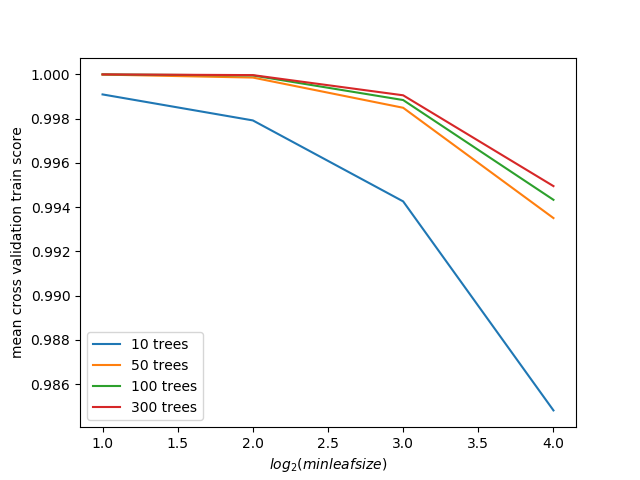
\includegraphics[width=\textwidth]{CVtestVsLeafSize.png}
    \end{minipage}
\caption{\footnotesize
(A,B) Cross Validation of Hyper-parameters for (A) training data and (B) testing data by contrasting mean cross validation score and $\log_2(minleafsize)$ giving the minimum leaf threshold as a measure of complexity. The scores for varying numbers of trees are shown.}
\end{figure}

\end{frame}
%-----------------------------------------------------------------
\begin{frame}[fragile]{Random Forest}
\small
\textbf{Cross-Validation and Results}

\medskip

The $\log_2(\text{minleafsize})$ which inversely measures the complexity suggests the more complex models performs outstandingly against the training data but has little impact on the testing data, a symptom of overfitting.

\vspace{3.75mm}

Adding trees has a similar positive affect on both datasets, however, also decreases exponentially as more trees are added. These results suggest that our model suffers from extreme levels of overfitting.

\vspace{3.75mm}
\begin{framed}
\centering
Our Kaggle submission of 300 trees and a minimum leaf number of 2 gave a prediction rate of 96.6\%
\end{framed}
\end{frame}
%-----------------------------------------------------------------
\begin{frame}{Multi-Layer Perceptron Classifier}
\textbf{Contrasting Gradient Descent Algorithms}
\vspace{3.75mm}

A Multi-layer Perceptron (MLP) is a type of deep neural network that is trained using backpropogation. An MLP consists of at least one hidden layer, an input/features layer, and an output/targets layer
\vspace{3.75mm}

For our MLP, we contrast stochastic gradient descent (SGD) and Adaptive Moment Estimation gradient descent (Adam GD)

\vspace{3.75mm}

\end{frame}
%-----------------------------------------------------------------
%\begin{frame}{Multi-Layer Perceptron Classifier}
%\tiny
%\textbf{Adam Parameter Estimation}
%
%\begin{itemize}
	%\item Exponentially decaying averages of the past gradient $\nabla_\theta f_t(\theta_{t-1})$ and
	%square of the gradient $\nabla_\theta f_t(\theta_{t-1})^2$ are stored as estimates of the first
	%and second moment of the gradient (mean $m_t$ and variance $v_t$ respectively).
	%\item The exponential decay rates $\beta_1$ and $\beta_2$ are initialized (generally near 1)\footnote{The
	%developers recommended default is $\beta_1 = 0.9$ and $\beta_2 = 0.999$. [3]} such that the moments can be
	%more specifically calculated using the following:
	%\begin{align*}
	%m_t \leftarrow& \beta_1 \cdot m_{t-1} + (1-\beta_1)\cdot \nabla_\theta f_t(\theta_{t-1})\\
	%v_t \leftarrow& \beta_2 \cdot v_{t-1} + (1-\beta_2)\cdot \nabla_\theta f_t(\theta_{t-1})^2
	%\end{align*}
	%\item With the initial $m_0$ and $v_0$ set to 0. In order to correct for bias, the following bias-corrected
	%moments are then computed:
	%\begin{align*}
	%\hat{m_t} \leftarrow& m_t/(1-\beta_1^t)\\
	%\hat{v_t} \leftarrow& v_t/(1-\beta_2^t)
	%\end{align*}
	%\item With $\beta_1^t$ and $\beta_2^t$ indicating $\beta_1$ and $\beta_2$ to the power of $t$.
	%Given some $\alpha$ and $\epsilon$ as regularization parameters, the parameters $\theta_t$ are then
	%updated using the following:
	%\begin{align*}
	%\theta_t \leftarrow& \theta_{t-1} - \alpha \cdot \hat{m_t}/(\sqrt{\hat{v_t}+\epsilon})
	%\end{align*}
	%\item This process is repeated until $\theta$ converges [3].
%\end{itemize}
%
%\end{frame}
%-----------------------------------------------------------------
\begin{frame}{Multi-Layer Perceptron Classifier}
    \textbf{Optimizing SGD}
    \includegraphics[width=0.9\textwidth]{patho.png}
\end{frame}
%-----------------------------------------------------------------
\begin{frame}{Multi-Layer Perceptron Classifier}
\small
\textbf{Implementation}

\medskip

In addition to our gradient descent algorithm, the following hyper-parameters were also varied:
\begin{itemize}
	\item Hidden Nodes: 128, 256, and 512
	\item Hidden Layers: 1 and 2
	\item Regularization Parameter ($\alpha$): 0.5, 0.1, 0.001, and 0.0001
\end{itemize}
\medskip
%Adam GD regularization parameters were initialized at the developer's (Kingma and Lei Ba) recommended defaults:
%\begin{itemize}
	%\item $\epsilon = 10^{-8}$
	%\item $\beta_1=0.9$
	%\item $\beta_2=0.999$ [3]
%\end{itemize}
%\medskip
The learning rate was not varied, instead an adaptive rate was chosen %which divides the current learning rate by 5 with a starting value of $0.001

\medskip

Once the code was prepared, training took approximately 46 minutes per model. Total training time took approximately 20 hours.

\end{frame}
%-----------------------------------------------------------------
\begin{frame}{Multi-Layer Perceptron Classifier}

\begin{figure}[h]
    \centering
    \begin{minipage}[t]{0.45\textwidth}
        \centering
        \textbf{(A)}
        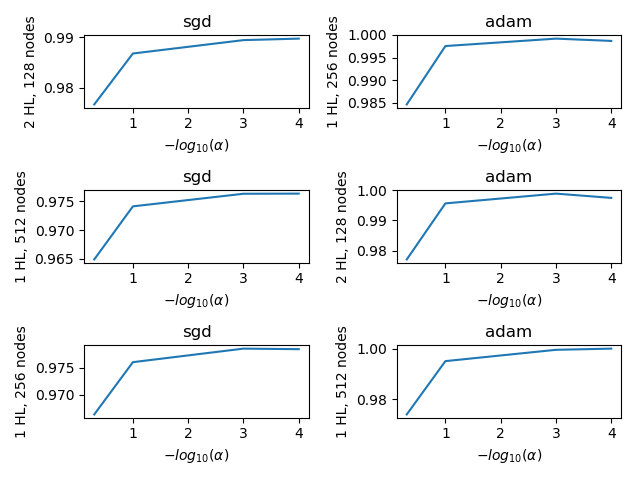
\includegraphics[width=\textwidth]{TrainscoreVsAlpha.png}
    \end{minipage}
    \begin{minipage}[t]{0.45\textwidth}
        \centering
        \textbf{(B)}
        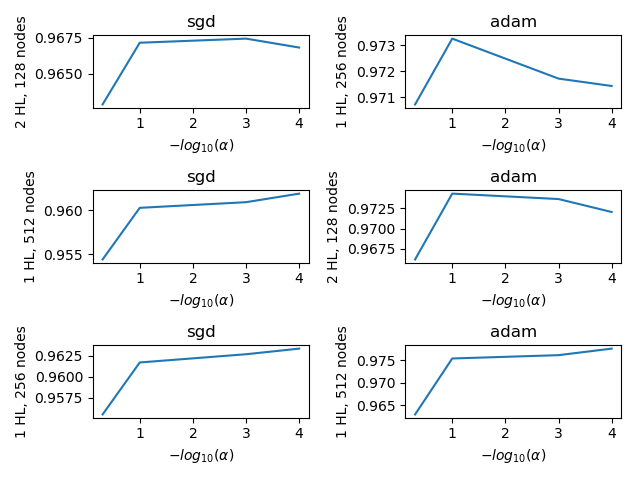
\includegraphics[width=\textwidth]{CVscoreVsAlpha.png}
    \end{minipage}
\caption{\scriptsize
(A,B) Cross Validation of Hyper-parameters for (A) training data and (B) testing data by contrasting the mean CVS in (A) and the prediction accuracy in (B) with $-\log_{10}(\alpha)$ giving a measure of complexity. For both (A) and (B), the left colomn gives the results for SGD, and the right colmn gives the results for Adam GD.}
\end{figure}

\end{frame}
%-----------------------------------------------------------------
\begin{frame}[fragile]{Multi-Layer Perceptron Classifier}
\scriptsize
\textbf{Cross-Validation and Results}

\smallskip

\begin{itemize}
	\item Training and cross-validation was done using \verb+model_selection.GridSearchCV+.
	\item The measure of complexity is given by $-\log_{10}(\alpha)$, meaning lower $\alpha$ values
	correspond to higher complexity.
\end{itemize}
\medskip
As expected, Adam gradient descent was the clear winner across the board.

Note:
\begin{itemize}
	\item Smaller $\alpha$ values (that is the larger $-\log_{10}(\alpha)$ values) almost consistently
	improves the prediction rate in (A), but for (B) in some cases causes severe prediction penalties.
	\item The most obvious example of this is at 1 HL and 256 nodes in (B).
\end{itemize}
\medskip

Our "winning" model with 1 HL and 512 nodes preformed rather consistently between training and testing datasets.

\medskip
\begin{framed}
\centering
The Kaggle submission of this model gave a prediction rate of 97.90\%.
\end{framed}
\end{frame}
%-----------------------------------------------------------------
\begin{frame}{Conclusions}

Overall, our MLP preformed better on the MNIST dataset
% As expected, our MLP was better suited for handwritten digit recognition. The high-dimensionality of the MNIST dataset provides a difficult hurdle for any RF, however possible improvements could be made to our current model.
\vspace{3.5mm}

Data processing to reduce dimensionality and tuning tree depth to add an additional constraint on model complexity could improve the classification accuracy of our RF. %Previous studies have shown that models clearly overfit for large depth values. Redeveloping our model to consider both the tree depth and the minimum number of leaves would put a stronger constraint on model complexity. While more difficult to implement, data processing to reduce dimensionality could be very effective.
\vspace{3.5mm}

Even with improvements to our RF, neural network architectures are still better suited for computer vision problems. % While it's likely the former changes to our RF will improve it's classification accuracy at a fraction of the MLP's training time, it's classification time will still suffer. Overall, computer vision problems are still better left in the hands of NN's and similar models.

\end{frame}
%-----------------------------------------------------------------
\begin{frame}[fragile]{References}

\tiny

[1] Bernard, S., Adam, S., \& Heutte, L. (2007). \textit{Using Random Forests for Handwritten Digit Recognition}. Ninth International Conference on Document Analysis and Recognition (ICDAR 2007) Vol 2. doi:10.1109/icdar.2007.4377074

\vspace{3mm}

[2] Hastie, T., Tibshirani, R., \& Friedman, J. H. (2017). The Elements of Statistical Learning: Data Mining, Inference, and Prediction. New York, NY: Springer.

\vspace{3mm}

[3] Kingma, D. P., \& Lei Ba, J. (2015).
\textit{Adam: A Method for Stochastic Optimization}. Conference Paper at ICLR. Retrieved from https://arxiv.org/abs/1412.6980.

\vspace{3mm}

[4] Pedregosa \textit{et al} (2011) \textit{Scikit-learn: Machine Learning in Python}. JMLR 12, pp. 2825-2830.

\vspace{3mm}

[5] Robnik-Šikonja, M. (2004). \textit{Improving Random Forests.} Machine Learning: ECML 2004 Proceedings, Springer, Berlin, 359-370.

\vspace{3mm}

[6] Y. LeCun \textit{et al} (1995) \textit{Learning Algorithms For Classification: A Comparison On Handwritten Digit Recognition}, in Oh, J. H. and Kwon, C. and Cho, S. (Eds), Neural Networks: The Statistical Mechanics Perspective, 261-276, World Scientific.

\end{frame}
%-----------------------------------------------------------------
\begin{frame}
	\begin{center}
	\begingroup
	\huge
	Thank You!\\
	\endgroup
	\end{center}
\end{frame}
%-----------------------------------------------------------------
\end{document}
